In diesem Unterkapitel wird die Größe des Target-Datensatzes signifikant reduziert, sodass lediglich noch 240 Stichproben zur Verfügung stehen. 
Die gleichen Tests wie im vorherigen Abschnitt werden erneut durchgeführt.

\begin{figure}[htpb]
    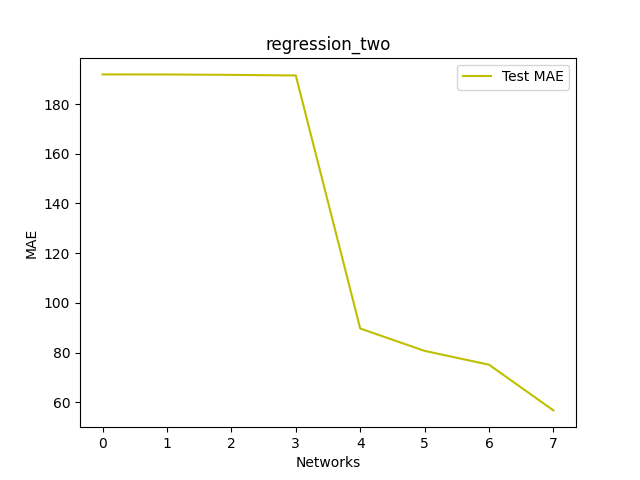
\includegraphics[height=5cm]{../../Plots/ba_plots/regression_small/regr2_ts.png}
    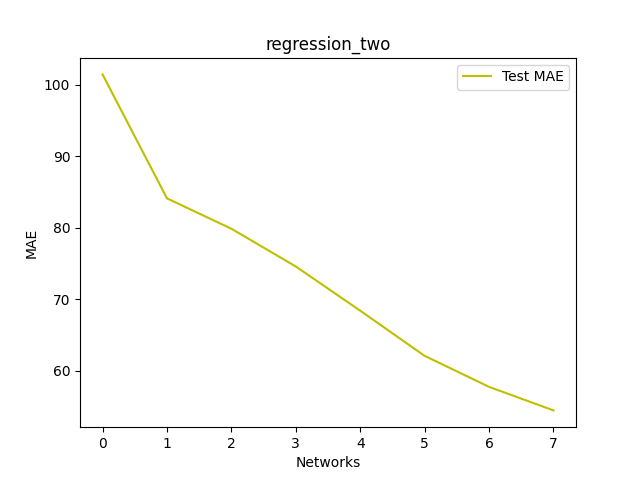
\includegraphics[height=5cm]{../../Plots/ba_plots/regression_small/woregr2_ts.png}
    \caption{\label{fig:smallregr} 
    \small{Abgebildet ist der Vergleich des Regr2-Netzwerks mit und ohne TF bei geringer Verfügbarkeit von Target-Daten. Die Tests entsprechen 
    links Regr2:TF4/240/10/8 und rechts Regr2:240/10/8. Dabei zeigt sich, dass das Netzwerk ohne TF eine bessere Performanz 
    erzielt als mit.}}
\end{figure}

Abbildung \ref{fig:smallregr} zeigt die Ergebnisse des Deep Cascade Netzwerks. Tatsächlich erzielt das Netzwerk ohne TF eine 
bessere Performanz als mit TF. Dies ist darauf zurückzuführen, dass die Gewichte der ersten Netzwerkhälfte primär auf dem 
Source-Datensatz optimiert wurden und somit weniger gut auf den Target-Datensatz übertragbar sind. 
Eine effektive Anpassung auf dem Target-Datensatz ist ebenfalls nicht möglich, da dieser eine unzureichende Anzahl an Stichproben enthält. 
Deep Cascade mit aktiviertem TF ist jedoch in einem Leistungsbereich, der eine praktische Nutzung weiterhin rechtfertigt.

Da sich die Ergebnisse deutlich von denen des Direct Cascade unterscheiden, wird im Folgenden die andere Netzwerkarchitektur betrachtet.

\begin{figure}[htpb]
    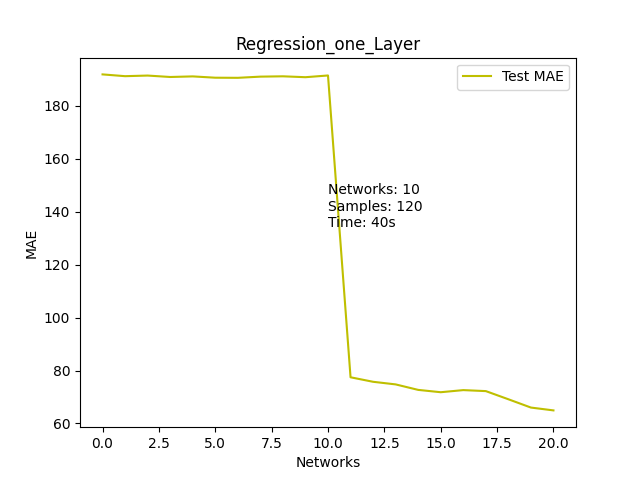
\includegraphics[height=5cm]{../../Plots/ba_plots/regression_small/onelayer_ts.png}
    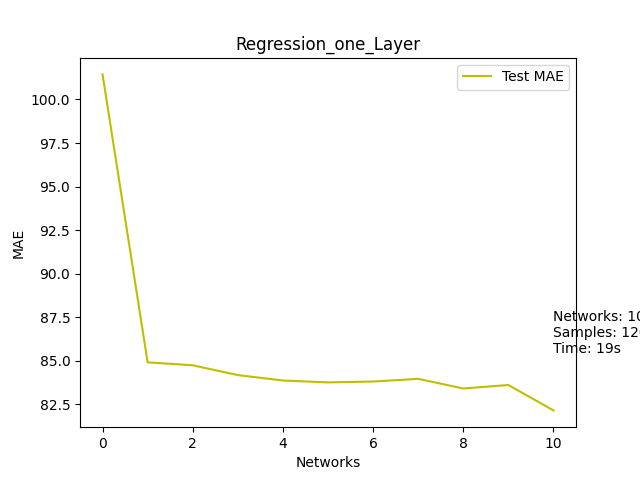
\includegraphics[height=5cm]{../../Plots/ba_plots/regression_small/woonelayer_ts.png}
    \caption{\label{fig:smallonl} 
    \small{Die Abbildung zeigt den Vergleich des 1Lay-Netzwerks im Szenario mit geringer Anzahl an Target-Daten, jeweils mit und ohne TF. Die 
    zugrunde liegenden Tests lauten: links 1Lay:TF11/240/10/21 und rechts 1Lay:240/10/11. Auffällig ist, dass in diesem Fall das Netzwerk mit 
    TF eine bessere Leistung erzielt als ohne.}}
\end{figure}

Abbildung \ref{fig:smallonl} zeigt die Ergebnisse des Direct Cascade Netzwerks. Es wird deutlich, dass diese Kaskadierungsvariante ohne TF eine 
signifikant schlechtere Leistung erzielt als mit TF. Dies weist auf einen positiven Transfer hin: Die Predicitons, die mithilfe des 
Source-Datensatzes auf bisher unberücksichtigte Target-Daten generiert werden, tragen zur Verbesserung der Gesamtergebnisse bei. Dadurch steht zu 
Beginn des Trainings auf dem Target-Datensatz eine größere Menge an Daten pro Stichprobe zur Verfügung. Diese zusätzlichen Informationen wirken 
sich nicht negativ auf die Modellleistung aus, sodass das Training mit TF insgesamt bessere Resultate liefert. 
Das Direct Cascade Netzwerk zeigt mit aktiviertem TF eine mit dem vollständigen Netzwerk etwas schlechtere, aber vergleichbare Performanz und 
erfüllt somit die Anforderungen für eine praxisnahe Anwendung.

Das Deep Cascade Netzwerk erreicht hingegen unabhängig vom Einsatz von TF eine leicht bessere Performanz. Dieser Unterschied könnte jedoch auch 
auf die abweichende Netzwerkarchitektur zurückzuführen sein, da die Layer-Strukturen nicht vollständig identisch sind. 
Dies könnte jedoch darauf zurückzuführen sein, dass die Gewichtungen der initialen Layer das Lernen auf dem Target-Datensatz nur geringfügig 
beeinflussen und die relevanten Merkmalsrepräsentationen primär in den nachfolgenden Hidden Layers erlernt werden können.

Die besten Ergebnisse liefert schließlich die Variante ohne Kaskadierung und ohne TF, bei der ein vollständiges Netzwerk direkt 
auf dem Ziel-Datensatz trainiert wurde, wie in Abbildung \ref{fig:smallonlcomp} dargestellt.

\begin{figure}
    \centering
    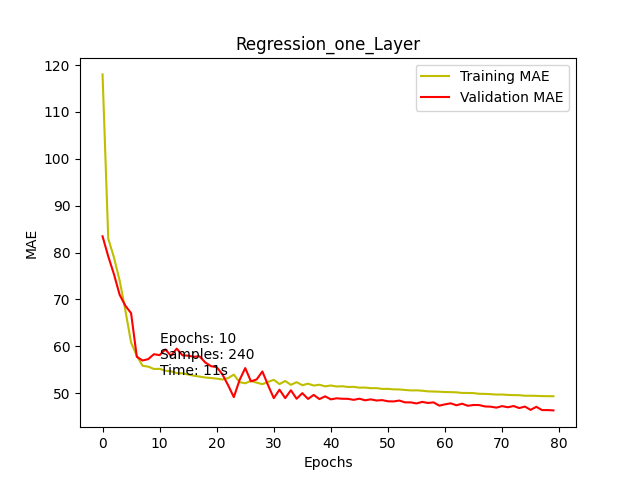
\includegraphics[height=5cm]{../../Plots/ba_plots/regression_small/onelayer_complete.png}
    \caption{\label{fig:smallonlcomp} 
    \small{Dem dargestellten Plot liegt der Test 1Lay:Comp/240//8 zugrunde. Trotz der geringen Anzahl an verfügbaren Daten erzielt dieses Modell 
    bessere Ergebnisse als alle anderen getesteten Varianten – obwohl es weder Kaskadierung noch TF verwendet.}}
\end{figure}

Der MAE-Wert auf den Testdaten liegt in diesem Fall bei etwa 53.000 US-Dollar, während er bei den Kaskadennetzwerken 
üblicherweise im Bereich von 60.000 bis 80.000 US-Dollar anzusiedeln ist.

Ein neuronales Netzwerk ohne Kaskadierung, jedoch mit einer hohen Anzahl an Hidden Layers und einem einzigen Trainingsdurchlauf über 80 Epochen, 
zeigt selbst bei geringer Datenmenge eine bessere Leistung als Netzwerke mit Kaskadierung. Es erreicht zudem nahezu den Fehlerwert, der bei 
einem deutlich größeren Trainingsdatensatz erzielt wird.

Im Gegensatz zu den anderen Netzarchitekturen besitzt dieses Modell die Fähigkeit, zwischen den Layern zu lernen und unvollständig verarbeitete 
Eingabedaten für die weitere Verarbeitung heranzuziehen. Dies dürfte maßgeblich zur verbesserten Modellperformanz beitragen.

Wird die Evaluation mit einem explizit großen Testdatensubset durchgeführt, so verschlechtert sich der absolute MAE-Wert bei allen Tests 
geringfügig. Die relativen Leistungsunterschiede zwischen den verschiedenen Netzarchitekturen bleiben jedoch unverändert.

Die Anwendung von TF ist sowohl in Kombination mit Deep Cascade als auch mit Direct Cascade möglich, wobei in beiden Fällen eine akzeptable 
Performanz erzielt werden kann. Für den praktischen Einsatz erscheinen daher beide Varianten grundsätzlich geeignet. Es ist jedoch 
empfehlenswert, weitere Untersuchungen mit deutlich kleineren Datensätzen durchzuführen, da bisher primär die Kaskadennetze einen 
Qualitätsverlust zeigten, wenn von großen auf kleinere Datenmengen umgestellt wurde.
